\section{Datasets and Distance Functions}
\label{sec:datasets-and-distance-functions}

Provide details on the datasets we use for benchmarks.

Add interesting t-SNE or UMAP embeddings of datasets.
For example~\ref{fig:discussion:umap-annthyroid-euclidean}

\begin{figure}[ht!]
    \centering
    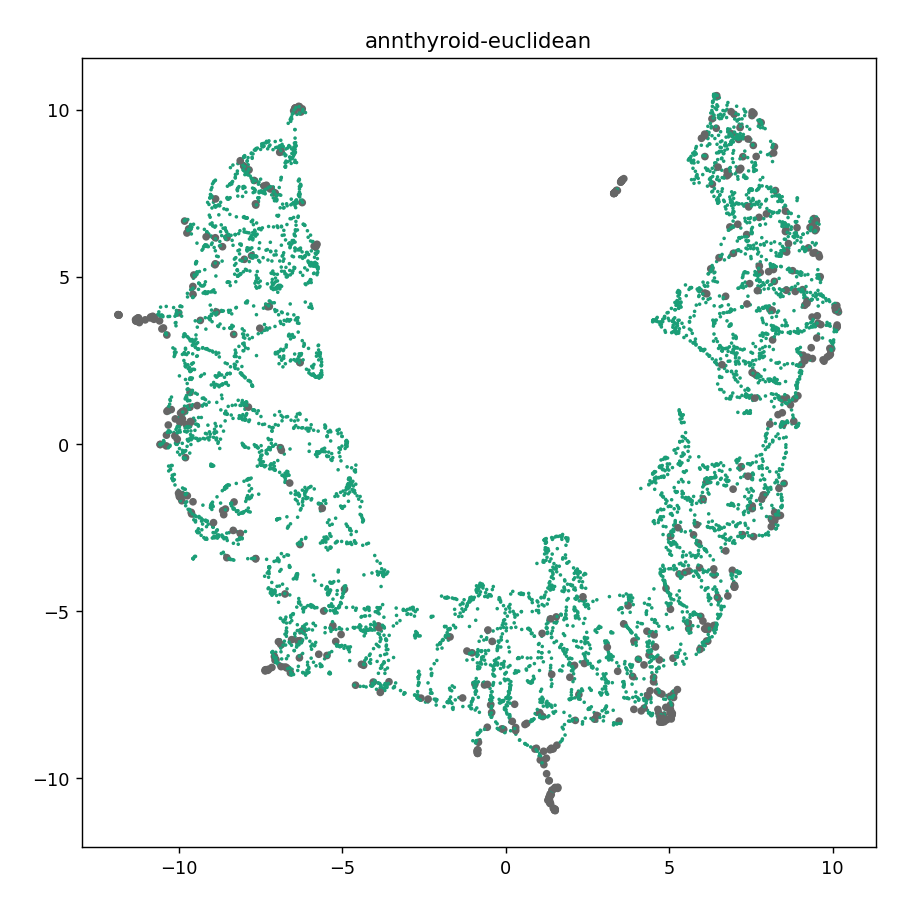
\includegraphics[width=2.5in]{images/umaps/annthyroid-euclidean-umap2d.png}
    \caption{UMAP embedding of Annthyroid data with the Euclidean distance function.}
    \label{fig:discussion:umap-annthyroid-euclidean}
\end{figure}

\subsection{APOGEE-2}
\label{subsec:datasets:apogee-2}
The Sloan Digital Sky Survey (SDSS) [3] Apache Point Observatory Galaxy Evolution
Experiment (APOGEE) [4] contains near-infrared
spectra of approximately 130,000 stellar objects in the Milky
Way galaxy. Each spectral datum describes a star's flux in
Janskys ($1 Jy = 10^{-26} W \dot m^{-2} \dot Hz^{-1}$) at each of 8,575 wavelengths ranging from $\lambda$ = 1.51 µm to 1.70 µm. Thus,
Thus, each datum is a real-valued vector in $\mathbb{R}_{+}^{8575}$. 

Astronomers use these near-infrared spectra to achieve a better understanding of our galaxy's history. 

TODO: Add details about why this dataset is a good candidate for CAKES.
TODO: Talk about distance functions used with this dataset: euclidean, cosine, Wasserstein-1d

\subsection{MaNGA}
\label{subsec:datasets:manga}
SDSS's Mapping Nearby Galaxies at APO (MaNGA) [CITE] contains spectral measurements across the face of each of 
about 10,000 galaxies across 2,700 deg$^2$. 

Like APOGEE, MaNGA helps astronomers understand the history of galaxies throughout their entire lifespan. 

TODO: Add details about why this dataset is a good candidate for CAKES. 
TODO: Talk about distance functions used with this dataset: euclidean, cosine, Wasserstein-2d

\subsection{Silva 18S}
\label{subsec:datasets:silva-18s}

TODO: Which Silva dataset exactly are we using and what is its cardinality and dimensionality?

TODO: Add details about why this dataset is a good candidate for CAKES.
TODO: Talk about distance functions used with this dataset: hamming, levenshtein

\dots

\subsection{ANN-Benchmarks suite}
\label{subsec:datasets:ann-benchmarks-suite}

deep1b: cosine

fashion-mnist: euclidean

gist: euclidean

glove: cosine

kosarak: jaccard

mnist: euclidean

nytimes: cosine

sift: euclidean

last.fm: cosine

\dots
